\clearpage
\section{بخش چهارم: بصری‌سازی بهینه‌سازی (\lr{Optimization Visualization})}

\begin{stepbox}
\field{مسئله‌ی پیش‌بینی قیمت خودرو و گرادیان کاهشی (\lr{Gradient Descent})}{
در این بخش، هدف برازش یک مدل رگرسیون خطی به صورت $y = ax + b$ بر روی مجموعه داده‌ی خودروهای دست‌دوم (\lr{Kaggle Used Cars}) جهت پیش‌بینی قیمت ($y$) بر اساس میزان کارکرد ($x$) است. الگوریتم گرادیان کاهشی و محاسبات مشتقات جزئی تابع زیان میانگین مربعات خطا (\lr{MSE Loss}) به صورت دستی پیاده‌سازی شده‌اند.
}
\end{stepbox}

\begin{codebox}[پیش‌پردازش داده‌ها و بهینه‌سازی الگوریتم گرادیان کاهشی]
\begin{lstlisting}[language=Python]
# 1. لگاریتم‌گیری و استانداردسازی داده‌ها
x_raw = np.log1p(df["odometer"].to_numpy(dtype=np.float64))
y_raw = np.log1p(df["price"].to_numpy(dtype=np.float64))

x = (x_raw - x_raw.mean()) / (x_raw.std() + 1e-12)
y = y_raw

# 2. محاسبه تابع زیان MSE و گرادیان‌ها
def mse_loss(a, b, x, y):
    return np.mean((a * x + b - y)**2)

def grads(a, b, x, y):
    e = (a * x + b) - y
    da = (2.0 / len(x)) * np.sum(e * x)
    db = (2.0 / len(x)) * np.sum(e)
    return da, db

# 3. حلقه بهینه‌سازی
a, b, lr = 0.0, 0.0, 0.1
for t in range(300):
    da, db = grads(a, b, x, y)
    a = a - lr * da
    b = b - lr * db
\end{lstlisting}
\end{codebox}

\begin{warnbox}[نقش استانداردسازی در همگرایی گرادیان]
عدم استانداردسازی داده‌های ورودی باعث می‌شود سطوح هم‌تراز تابع زیان به شدت کشیده (\lr{Ill-conditioned}) شوند که منجر به نوسانات شدید یا انفجار گرادیان‌ها (\lr{Exploding Gradients}) می‌گردد. با اعمال (\lr{Z-Score Normalization})، رویه‌ی زیان به صورت کروی هموار درآمده و امکان استفاده از نرخ یادگیری (\lr{Learning Rate}) بزرگتر جهت همگرایی سریع‌تر فراهم می‌شود.
\end{warnbox}

\subsection{تحلیل نتایج بهینه‌سازی و همگرایی}

\begin{figure}[htbp]
    \centering
    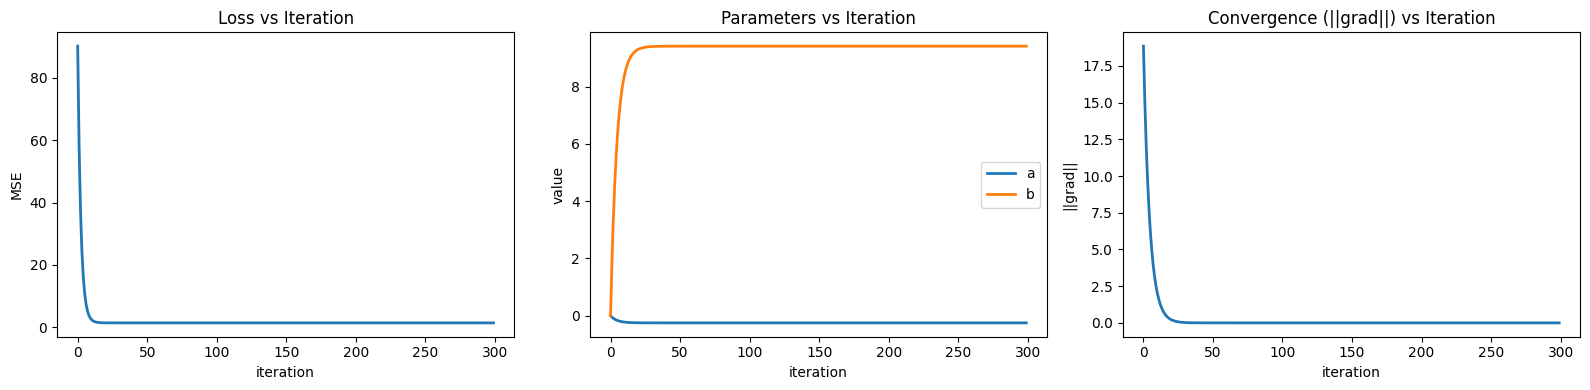
\includegraphics[width=1\textwidth]{images/img_optimization.png}
    \caption{نمودارهای تغییرات تابع زیان (\lr{MSE})، روند تغییر پارامترها ($a, b$) و هنجار بردار گرادیان ($||\nabla L||_2$)}
    \label{fig:optim_plots}
\end{figure}

\begin{stepbox}
\field{تفسیر نتایج و تحلیل رفتار گرادیان}{
\textbf{۱. روند همگرایی زیان (\lr{Loss}):} \\
نمودار زیان به صورت یکنواخت نزولی بوده و پس از طی تکرارهای اولیه به تثبیت می‌رسد که نشان‌دهنده انتخاب مناسب نرخ یادگیری ($\eta = 0.1$) و حرکت صحیح در خلاف جهت گرادیان است.

\textbf{۲. هنجار گرادیان ($||\nabla L||_2$):} \\
نمودار هنجار بردار گرادیان ($\sqrt{da^2 + db^2}$) با نزدیک شدن مدل به نقطه کمینه (\lr{Minimum}) به صفر میل می‌کند که اثبات ریاضی رسیدن به نقطه بهینه موضعی است.

\textbf{۳. تفسیر شیب خط ($a = -0.25$):} \\
مقدار به‌دست‌آمده برای پارامتر $a$ منفی است که نشان‌دهنده‌ی وجود **رابطه‌ی معکوس** بین کارکرد خودرو و قیمت آن است. به عبارت دیگر، با افزایش میزان کارکرد، قیمت خودرو طبق نرخ به‌دست‌آمده افت می‌کند.
}
\end{stepbox}